%!TeX encoding = UTF-8
%!TeX program = xelatex
\documentclass[notheorems, aspectratio=54]{beamer}
% aspectratio: 1610, 149, 54, 43(default), 32
\usepackage{url}
\usepackage{qrcode}
\usepackage{xcolor,lipsum}
\usepackage{latexsym}
\usepackage{amsmath,amssymb}
\usepackage{mathtools}
\usepackage{color,xcolor}
\usepackage{graphicx}
\usepackage{algorithm}
\usepackage{amsthm}
\usepackage{lmodern} % 解决 font warning
% \usepackage[UTF8]{ctex}
\usepackage{animate} % insert gif

\usepackage{lipsum} % To generate test text
\usepackage{ulem}
\usepackage{listings} % display code on slides; don't forget [fragile] option after \begin{frame}
\usepackage{listings-rust}
% ----------------------------------------------
% tikx
\usepackage{framed}
\usepackage{tikz}
\usepackage{pgf}
\texorpdfstring{}{}
\usetikzlibrary{calc,trees,positioning,arrows,chains,shapes.geometric,%
    decorations.pathreplacing,decorations.pathmorphing,shapes,%
    matrix,shapes.symbols}
\pgfmathsetseed{1} % To have predictable results
% Define a background layer, in which the parchment shape is drawn
\pgfdeclarelayer{background}
\pgfsetlayers{background,main}

% define styles for the normal border and the torn border
\tikzset{
  normal border/.style={black!70!gray, decorate,
     decoration={random steps, segment length=2.5cm, amplitude=.7mm}},
  torn border/.style={black!70!gray, decorate,
     decoration={random steps, segment length=.5cm, amplitude=1.7mm}}}

% Macro to draw the shape behind the text, when it fits completly in the
% page
\def\parchmentframe#1{
\tikz{
  \node[inner sep=2em] (A) {#1};  % Draw the text of the node
  \begin{pgfonlayer}{background}  % Draw the shape behind
  \fill[normal border]
        (A.south east) -- (A.south west) --
        (A.north west) -- (A.north east) -- cycle;
  \end{pgfonlayer}}}

% Macro to draw the shape, when the text will continue in next page
\def\parchmentframetop#1{
\tikz{
  \node[inner sep=2em] (A) {#1};    % Draw the text of the node
  \begin{pgfonlayer}{background}
  \fill[normal border]              % Draw the ``complete shape'' behind
        (A.south east) -- (A.south west) --
        (A.north west) -- (A.north east) -- cycle;
  \fill[torn border]                % Add the torn lower border
        ($(A.south east)-(0,.2)$) -- ($(A.south west)-(0,.2)$) --
        ($(A.south west)+(0,.2)$) -- ($(A.south east)+(0,.2)$) -- cycle;
  \end{pgfonlayer}}}

% Macro to draw the shape, when the text continues from previous page
\def\parchmentframebottom#1{
\tikz{
  \node[inner sep=2em] (A) {#1};   % Draw the text of the node
  \begin{pgfonlayer}{background}
  \fill[normal border]             % Draw the ``complete shape'' behind
        (A.south east) -- (A.south west) --
        (A.north west) -- (A.north east) -- cycle;
  \fill[torn border]               % Add the torn upper border
        ($(A.north east)-(0,.2)$) -- ($(A.north west)-(0,.2)$) --
        ($(A.north west)+(0,.2)$) -- ($(A.north east)+(0,.2)$) -- cycle;
  \end{pgfonlayer}}}

% Macro to draw the shape, when both the text continues from previous page
% and it will continue in next page
\def\parchmentframemiddle#1{
\tikz{
  \node[inner sep=2em] (A) {#1};   % Draw the text of the node
  \begin{pgfonlayer}{background}
  \fill[normal border]             % Draw the ``complete shape'' behind
        (A.south east) -- (A.south west) --
        (A.north west) -- (A.north east) -- cycle;
  \fill[torn border]               % Add the torn lower border
        ($(A.south east)-(0,.2)$) -- ($(A.south west)-(0,.2)$) --
        ($(A.south west)+(0,.2)$) -- ($(A.south east)+(0,.2)$) -- cycle;
  \fill[torn border]               % Add the torn upper border
        ($(A.north east)-(0,.2)$) -- ($(A.north west)-(0,.2)$) --
        ($(A.north west)+(0,.2)$) -- ($(A.north east)+(0,.2)$) -- cycle;
  \end{pgfonlayer}}}

% Define the environment which puts the frame
% In this case, the environment also accepts an argument with an optional
% title (which defaults to ``Example'', which is typeset in a box overlaid
% on the top border
\newenvironment{parchment}[1][Example]{%
  \def\FrameCommand{\parchmentframe}%
  \def\FirstFrameCommand{\parchmentframetop}%
  \def\LastFrameCommand{\parchmentframebottom}%
  \def\MidFrameCommand{\parchmentframemiddle}%
  \vskip\baselineskip
  \MakeFramed {\FrameRestore}
  \noindent\tikz\node[inner sep=1ex, draw=black!20, fill=black!90,
          anchor=west, overlay] at (0em, 2em) {\sffamily#1};\par}%
{\endMakeFramed}

% ----------------------------------------------

\mode<presentation>{
    \usetheme{Warsaw}
    % Boadilla CambridgeUS
    % default Antibes Berlin Copenhagen
    % Madrid Montpelier Ilmenau Malmoe
    % Berkeley Singapore Warsaw
    \usecolortheme{seagull}
    % beetle, beaver, orchid, whale, dolphin, seagull
    \useoutertheme{infolines}
    % infolines miniframes shadow sidebar smoothbars smoothtree split tree
    \useinnertheme{circles}
    % circles, rectanges, rounded, inmargin
}

% ---------------------------------------------------------------------
% Jet Black Theme
\setbeamercolor{normal text}{fg=white,bg=black!90}
\setbeamercolor{structure}{fg=white}

\setbeamercolor{alerted text}{fg=red!85!black}

\setbeamercolor{item projected}{use=item,fg=black,bg=item.fg!35}

\setbeamercolor*{palette primary}{use=structure,fg=structure.fg}
\setbeamercolor*{palette secondary}{use=structure,fg=structure.fg!95!black}
\setbeamercolor*{palette tertiary}{use=structure,fg=structure.fg!90!black}
\setbeamercolor*{palette quaternary}{use=structure,fg=structure.fg!95!black,bg=black!80}

\setbeamercolor*{framesubtitle}{fg=white}

\setbeamercolor*{block title}{parent=structure,bg=black!70!gray}
\setbeamercolor*{block body}{fg=black,bg=black!10}
\setbeamercolor*{block title alerted}{parent=alerted text,bg=black!15}
\setbeamercolor*{block title example}{parent=example text,bg=black!15}
% ---------------------------------------------------------------------


% ---------------------------------------------------------------------
% flow chart
\tikzset{
    >=stealth',
    punktchain/.style={
        rectangle,
        rounded corners,
        % fill=black!10,
        draw=white, very thick,
        text width=6em,
        minimum height=2em,
        text centered,
        on chain
    },
    largepunktchain/.style={
        rectangle,
        rounded corners,
        draw=white, very thick,
        text width=10em,
        minimum height=2em,
        on chain
    },
    line/.style={draw, thick, <-},
    element/.style={
        tape,
        top color=white,
        bottom color=blue!50!black!60!,
        minimum width=6em,
        draw=blue!40!black!90, very thick,
        text width=6em,
        minimum height=2em,
        text centered,
        on chain
    },
    every join/.style={->, thick,shorten >=1pt},
    decoration={brace},
    tuborg/.style={decorate},
    tubnode/.style={midway, right=2pt},
    font={\fontsize{10pt}{12}\selectfont},
}
% ---------------------------------------------------------------------

% code setting
\lstset{
    language=C++,
    basicstyle=\ttfamily\footnotesize,
    keywordstyle=\color{red},
    breaklines=true,
    xleftmargin=2em,
    numbers=left,
    numberstyle=\color[RGB]{222,155,81},
    frame=leftline,
    tabsize=4,
    breakatwhitespace=false,
    showspaces=false,
    showstringspaces=false,
    showtabs=false,
    morekeywords={Str, Num, List},
}

% ---------------------------------------------------------------------

\newcommand{\reditem}[1]{\setbeamercolor{item}{fg=red}\item #1}

\newcommand*{\Scale}[2][4]{\scalebox{#1}{\ensuremath{#2}}}

\renewcommand\textbullet{\ensuremath{\bullet}}

% -------------------------------------------------------------

%% preamble
\title[Actor Model]{The Hitchhiker's Guide to The Actor Model in Rust}
% \subtitle{The subtitle}
\author[Ryan Kung]{
\includegraphics[height=2cm]{./ieee-blockchain.png} \\ Ryan J. Kung}

\institute[IEEE Blockchain]{ryankung@ieee.org}
% -------------------------------------------------------------
\begin{document}

% title frame
\begin{frame}
    \titlepage
\end{frame}

% normal frame
\section{Overview}

\begin{frame}
  \frametitle{Overview}
  \begin{itemize}
  \item Introduction to The Actor Model
     \begin{itemize}
     \item History of Actor Model
     \item Hierarchies in Actor Model
     \item Actor Model and Process Calculus
     \end{itemize}
   \item Introduction to Actix \& Actix-web
     \begin{itemize}
     \item Actor \& Arbiter
     \item Message and Handler
    \end{itemize}
    \item More trait Types in Actix
    \begin{itemize}
      \item SyncArbiter \& Supervised
    \end{itemize}
    \item Ghost in the Shell
    \begin{itemize}
      \item Tokio \& Futures
    \end{itemize}
  \item Issues \& Solutions
\end{itemize}
\end{frame}

\section{Introduction to The Actor Model}
\begin{frame}
  \frametitle{History of Actor Model}
  \begin{center}
    \bfseries{A Universal Modular ACTOR Formalism for Artificial Intelligence.}
  \end{center}
  \begin{center}
    Carl Hewitt,\  Peter Bishop,\ Richard Steiger\\
    in\\
    \bfseries{1973}
  \end{center}
  \begin {center}
  \end {center}

    \begin{center}
    \bfseries{Actor induction and meta-evaluation.}
  \end{center}
  \begin{center}
    Carl Hewitt,\  Peter Bishop,\ Irene Greif,\ Brian Smith,\ Todd Maston,\ Rechard Steiger\\
    in\\
    \bfseries{1973}
  \end{center}
  \begin {center}
  \end {center}
\end{frame}
\begin{frame}
  \frametitle{History of Actor Model}
  \begin{center}
    ``Our formalism shows how all of the modes of behavior can be defined in terms of one kind of behavior: Sending message to actors, An actor is always invoked uniformly in exactly the same way regardless of whether it behaves: As a recursive function, data structure, or process``\cite{actor}\cite{meta}
  \end{center}
\end{frame}

\begin{frame}
  \frametitle{History of Actor Model}
    \begin{center}
    ``It's van to multiply Entities beyond need. -- William of Occam``\\
    ``Monotheism is the Answer``\cite{actor}
  \end{center}
\end{frame}

\begin{frame}
  \frametitle{Hierarchies in Actor Model}
  \begin{itemize}
  \item {\bfseries Scheduling:}

    :- Every actor has a scheduler which determines when the actor actually acts after it is sent a message.
  \item {\bfseries Intentions:}

    :- Every actor has an intention which makes certain that the prerequisites and context of the actor being sent the message are satisfied.
  \item {\bfseries Monitoring:}

    :- Every actor can have monitors which look over each message sent to the actor.
  \item {\bfseries binding:}

    :- Every actor can have a procedure for looking up the values of names that occur within it.
  \item {\bfseries Resource Management:}

    :- Every actor has a banker which monitors the use of space and time.
  \end{itemize}
\end{frame}

\begin{frame}
  \frametitle{Actor Model and Process Calculus}
  There are numerous process calculi\cite{picalcu, historyofpi}, each of them are using difference abstract method and formalize Symbol. And they (the $Processes$ or $Agent$) usually sharing a $Channel$. Actually, we can also model the Actor Model with Algebra method, there existing some related work about it\cite{actoralgebra}.
  \begin{center}
    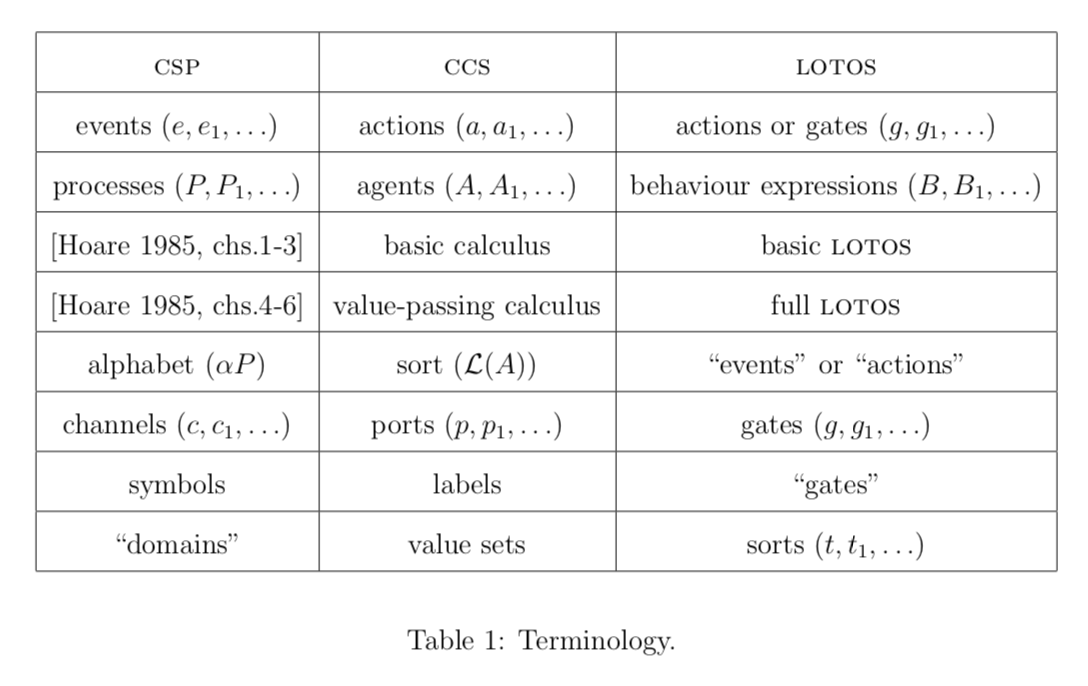
\includegraphics[height=4cm]{./pialgebra.png}
  \end{center}
\end{frame}
\section{Introduction to Actix \& Actix-web}
\begin{frame}
  \frametitle{Introduction to Actix \& Actix-web}
  \begin{center}
    
\includegraphics[height=3cm]{./actix.png}
  \end{center}
  Actix is a Actor Model implementation for Rust\cite{actix}, which is Blazingfy Fast (about 28x faster than flask\cite{bm}), Type Safe, and easy to use.
    \begin{center}
    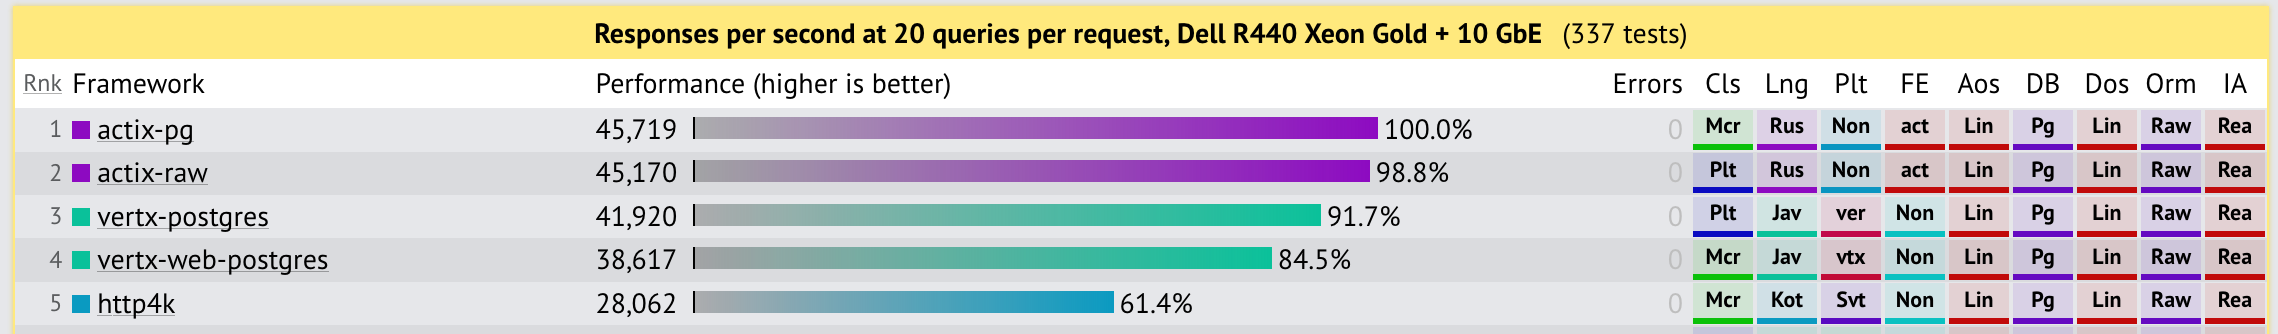
\includegraphics[height=1.2cm]{./bm.png}
  \end{center}

\end{frame}

\begin{frame}[fragile]
  \frametitle{Introduction to Actix \& Actix-web}
  \begin{lstlisting}[language=Rust]
extern crate actix_web;
use actix_web::{server, App, HttpRequest, Responder};

fn greet(req: &HttpRequest) -> impl Responder {
    let to = req.match_info().get("name").unwrap_or("World");
    format!("Hello {}!", to)
}
fn main() {
    server::new(|| {
        App::new()
            .resource("/", |r| r.f(greet))
            .resource("/{name}", |r| r.f(greet))
    })
    .bind("127.0.0.1:8000")
    .expect("Can not bind to port 8000")
    .run();
}

   \end{lstlisting}
 \end{frame}

\begin{frame}[fragile]
  \frametitle{Aribiter \& Actor}
  $Actor$ is the most basic trait of $actix$, which encapsulate state and behavior and defined as:
  \begin{lstlisting}[language=Rust]
    pub trait Actor: Sized + 'static {
      type Context: ActorContext;
      fn started(&mut self, ctx: &mut Self::Context)
      fn stopping(&mut self, ctx: &mut Self::Context)
      fn stopped(&mut self, ctx: &mut Self::Context)
      fn start(self) -> Addr<Self>
      fn create<F>(f: F) -> Addr<Self>
    }
  \end{lstlisting}
\end{frame}

\begin{frame}[fragile]
  \frametitle{Aribiter \& Actor}
  $Arbiter$ is Event loop controller, which is also a Actor implementation, Arbiter controls event loop in its thread. Each arbiter runs in separate thread. Arbiter provides several api for event loop access.

  \begin{lstlisting}[language=Rust]
    impl Arbiter {
      pub fn current() -> Addr<Arbiter>;
      pub fn spawn<F>(future: F);
      pub fn start<A, F>(f: F) -> Addr<A>
    }
  \end{lstlisting}
  And has follow $impl$s for controlling itself:
  \begin{itemize}
  \item $Actor$
  \item $Handler<StopArbiter>$
  \item $Handler<Execute<I, E>>$
  \end{itemize}
  Where $<StopArbbiter>$ and $<Execute<I, E>$ are impls of $Message$ trait.
\end{frame}


\begin{frame}[fragile]
  \frametitle{Message and Handler}
  The $Message$ and $Handler$ trait was defined as:
  \begin{lstlisting}[language=Rust]
  pub trait Message {
    type Result: 'static;
  }

  pub trait Handler<M>
  where Self: Actor,
        M: Message
  {
    type Result: MessageResponse<Self, M>;
    fn handle(&mut self, msg: M, ctx: &mut Self::Context) -> Self::Result;
  }
  \end{lstlisting}
\end{frame}

\begin{frame}[fragile]

  \frametitle{Message and Handler}
  \begin{lstlisting}[language=Rust]
struct MyActor { count: usize };
struct Ping(usize);

impl Actor for MyActor {
    type Context = Context<Self>;
}

impl Message for Ping {
    type Result = usize;
  }

impl Handler<Ping> for MyActor {
  type Result = usize;
  fn handle(&mut self, msg: Ping, ctx: &mut Context<Self>) -> Self::Result {
    self.count += msg.0;
    self.count
  }
}
  \end{lstlisting}
\end{frame}


\begin{frame}[fragile]

  \frametitle{Message and Handler}
  \begin{lstlisting}[language=Rust]
fn main() {
    let system = System::new("test");

    // start new actor
    let addr = MyActor{count: 10}.start();

    // send message and get future for result
    let res = addr.send(Ping(10));

    Arbiter::spawn(
        res.map(|res| {
            println!("RESULT: {}", res == 20);
        })
        .map_err(|_| ()));

    system.run();
}
\end{lstlisting}
\end{frame}


\section{More trait Types in Actix}

\begin{frame}[fragile]
  \frametitle{SyncArbiter}
  Sync actors could be used for cpu bound load.

  Only one sync actor runs within arbiter's thread. Sync actor process one message at a time. Sync arbiter can start multiple threads with separate instance of actor in each.
\end{frame}

\begin{frame}[fragile]
  \frametitle{SyncArbiter}
  By modified the $ping$ example:
    \begin{lstlisting}[language=Rust]
struct MyActor { count: usize };
struct Ping(usize);

impl Actor for MyActor {
    type Context = SyncContext<Self>;
}

impl Message for Ping {
    type Result = usize;
  }

impl Handler<Ping> for MyActor {
  type Result = usize;
  fn handle(&mut self, msg: Ping, ctx: &mut Context<Self>) -> Self::Result {
    self.count += msg.0;
    self.count
  }
}
  \end{lstlisting}

\end{frame}

\begin{frame}[fragile]
  \frametitle{SyncArbiter}
  And start 2 worker as Actor.
  \begin{lstlisting}[language=Rust]
fn main() {
    System::run(|| {
        let addr = SyncArbiter::start(2, || MyArbiter);
    });
}
  \end{lstlisting}

\end{frame}

\begin{frame}[fragile]
  \frametitle{Supervised}
  Supervisor is a event manager which handler $restart$ event for an $Actor$, and it's quiet useful for implementation an SystemRegistry(wont discuss here):
  \begin{lstlisting}[language=Rust]
impl actix::Supervised for MyActor {
    fn restarting(&mut self, ctx: &mut Context<MyActor>) {
        println!("restarting");
    }
}
  \end{lstlisting}

\end{frame}



\section{Ghost in the Shell}

\begin{frame}[fragile]
  \frametitle{Tokio \& Futures}
  A common usage of Actor Message calling is like this:
  \begin{lstlisting}[language=Rust]
  fn index(state: State<AppState>) -> FutureResponse<HttpResponse> {
    state
        .db
        .send(&some_msg)
        .from_err()
        .and_then(|res| mk_json_response(res))
        .responder()
      }
    \end{lstlisting}

    $fn\ and\_then$ is a method function of $ActorFuture$ trait, which is very similar to a regular Future.
    and also requied a $poll$ method:
    \begin{lstlisting}[language=Rust]
fn poll(
    &mut self,
    srv: &mut Self::Actor,
    ctx: &mut <Self::Actor as Actor>::Context
) -> Poll<Self::Item, Self::Error>
\end{lstlisting}
\end{frame}

\begin{frame}[fragile]
  \frametitle{Tokio \& Futures}
  After calling $and\_then$, it will return an $AndThen$ which was created by the $Future::and\_then$.
  \begin{lstlisting}[language=Rust]
  pub struct AndThen<A, B, F> where
    A: Future,
    B: IntoFuture,  { /* fields omitted */ }
  \end{lstlisting}
  Which is meaning that the event loop of $Arbiter$ is managing by Tokio and Futures.
\end{frame}

\begin{frame}[fragile]
  \frametitle{Tokio \& Futures}
  Let's go check what $actix$ actually did when spawn an $Arbiter$
  \begin{lstlisting}[language=Rust]
use tokio::executor::current_thread::spawn;
use tokio::runtime::current_thread::Builder as RuntimeBuilder;
impl ArbiterBuilder {
    fn new() -> Self {
        ArbiterBuilder {
            name: None,
            stop_system_on_panic: false,
            runtime: RuntimeBuilder::new(),
        }
}
  \end{lstlisting}
\end{frame}
\section{Issues \& Solutions}
\begin{frame}[fragile]
  \frametitle{No panic!}
\end{frame}

\begin{frame}[fragile]
  \frametitle{Towel Needed}
\end{frame}

\begin{frame}[allowframebreaks]
    \frametitle{Reference}
  \bibliographystyle{unsrt}
  \bibliography{slide}
\end{frame}
\begin{frame}
  \frametitle{Thanks}
  \begin{center}
    Programs should not only work, but they should appear to work as well.
    -- by PDP-1X Dogma
  \end{center}
  \begin{center}
    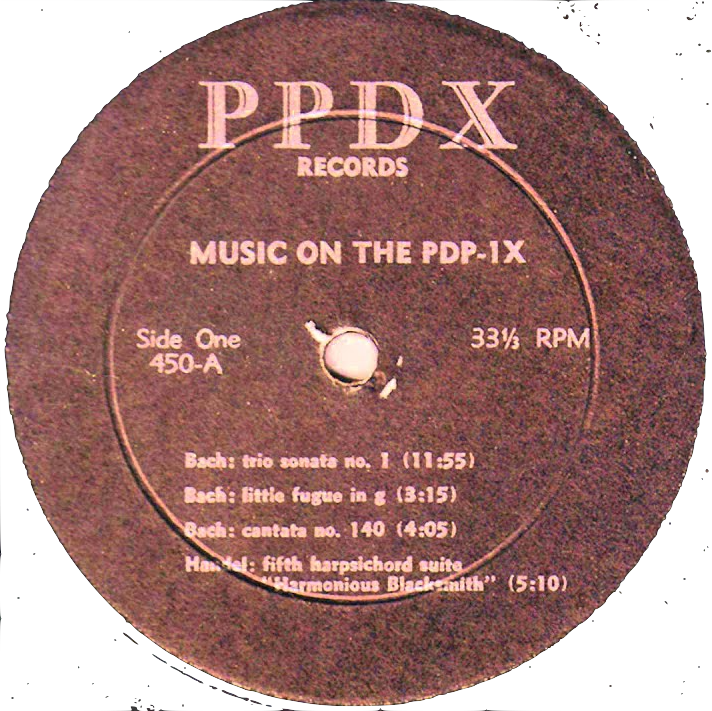
\includegraphics[height=6cm]{./maxresdefault.png}
  \end{center}
\end{frame}
\end{document}